\documentclass{article}
\usepackage{amsmath}
\usepackage{graphicx}

\usepackage[utf8]{inputenc}
\usepackage[colorlinks=true, linkcolor=blue, citecolor=black, backref=page]{hyperref}
\usepackage{lscape}
\usepackage{placeins}
\usepackage{listings}
\usepackage{xcolor}
\usepackage{float}
% Define custom colors
\definecolor{dkgreen}{rgb}{0,0.6,0}
\definecolor{gray}{rgb}{0.5,0.5,0.5}
\definecolor{mauve}{rgb}{0.58,0,0.82}

% Configure lstlisting settings for Python
\lstset{
  frame=tb,                      % Draw a frame at the top and bottom of the code block
  language=Python,               % Set the language to Python
  aboveskip=3mm,                 % Add space above the code block
  belowskip=3mm,                 % Add space below the code block
  showstringspaces=false,        % Do not display string spaces with special underlines
  columns=flexible,              % Allow flexible column spacing
  basicstyle={\small\ttfamily},  % Set the font style and size for code
  numbers=left,                  % Display line numbers on the left
  numberstyle=\tiny\color{gray}, % Style for line numbers
  keywordstyle=\color{blue},     % Style for keywords
  commentstyle=\color{dkgreen},  % Style for comments
  stringstyle=\color{mauve},     % Style for strings
  breaklines=true,               % Allow long lines to break
  breakatwhitespace=true,        % Break lines at whitespace if possible
  tabsize=4                      % Set tab size to 4 spaces
}


\begin{document}

\title{Task 4 -- NLO Lab Sheet 3}

\maketitle

\section{Solution to 4 - BFGS for the 5-dimensional \textit{chebyquad} problem}

\subsection{Mathematical Analysis}
The Hessian at the solution is approximately as follows:
$$
Q=\left(\begin{array}{ccccc}
22.4639 & -8.5053 & -1.8359 & 2.4924 & -1.5605 \\
-8.5053 & 8.6275 & -1.3643 & -4.7052 & 2.4924 \\
-1.8359 & -1.3643 & 11.2000 & -1.3639 & -1.8359 \\
2.4924 & -4.7052 & -1.3639 & 8.6273 & -8.5052 \\
-1.5605 & 2.4924 & -1.8359 & -8.5052 & 22.4639
\end{array}\right)
$$
The inverse of the final BFGS approximation is as follows:
$$
H_k^{-1}=\left(\begin{array}{ccccc}
26.60942 & -10.23183 & -4.63200 & 0.53008 & 1.38542 \\
-10.23183 & 10.20357 & 0.52151 & -5.02250 & 1.63645 \\
-4.63200 & 0.52151 & 15.02718 & -0.71726 & -4.20901 \\
0.53008 & -5.02250 & -0.71726 & 11.54647 & -11.32184 \\
1.38542 & 1.63645 & -4.20901 & -11.32184 & 26.51774
\end{array}\right)
$$





$H_k^{-1}$ is the approximation of the inverse of the Hessian $Q^{-1}$ and not $Q$ the Hessian of the objective function itself. $H_k$ is the BFGS approximation of $Q^{-1}$. Therefore, a correct comparison is between $Q^{-1}$ and $H_k$. Comparing $Q$ with $H_k^{-1}$ would be inappropriate since they are fundamentally different representations. 

I have provided a simple code below for the calculation of inverses of the above matrices, their eigenvalues and eigenvectors and have finally performed a principal component analysis which is just finding the angles between two eigenvectors. The PCA is just one of the methods to contrast two matrices where we try to essentially find the directions (eigenvectors) in which the data (matrix) has the largest variance (eigenvalue), other methods could just look at the magnitudes of Forbenius /Spectral norm. 

\subsection{Python Code for Inverse, Eigenvalue, Eigenvector and Angles}
\begin{lstlisting}

#One can directly use the code without any dependencies of the 15.py files that had been provided in Lab3.zip as I have defined the matrices here at the start and then used functions to operate them upon

import numpy as np
import matplotlib.pyplot as plt
from mpl_toolkits.mplot3d import Axes3D
from matplotlib import cm


class MatrixOperations:
    """
    A class to handle matrix operations such as eigenvalue/eigenvector computation
    and matrix inversion.
    """
    def __init__(self, matrix: np.ndarray):
        self.matrix = matrix
        self.eigenvalues, self.eigenvectors = np.linalg.eig(matrix)

    @staticmethod
    def calculate_angle(v1: np.ndarray, v2: np.ndarray) -> float:
        """
        Computes the angle (in degrees) between two vectors.
        """
        cos_theta = np.dot(v1, v2) / (np.linalg.norm(v1) * np.linalg.norm(v2))
        return np.degrees(np.arccos(np.clip(cos_theta, -1.0, 1.0)))

    def inverse(self) -> np.ndarray:
        """Returns the inverse of the matrix."""
        return np.linalg.inv(self.matrix)


def plot_eigenvectors_and_planes(vec1: np.ndarray, vec2: np.ndarray, pair_idx: int, angle: float) -> None:
    """
    Plots the eigenvectors as arrows, visualizes the plane they span, and the angle between them.
    """
    fig = plt.figure(figsize=(8, 6))
    ax = fig.add_subplot(111, projection='3d')

    # Create grid to visualize the plane spanned by the two vectors
    x = np.linspace(-1, 1, 10)
    y = np.linspace(-1, 1, 10)
    X, Y = np.meshgrid(x, y)
    Z = (vec1[0] * X + vec1[1] * Y) / vec2[2] if vec2[2] != 0 else np.zeros_like(X)

    # Plot the surface (the plane)
    ax.plot_surface(X, Y, Z, alpha=0.3, cmap=cm.coolwarm, edgecolor='none')

    # Plot the eigenvectors as arrows
    ax.quiver(0, 0, 0, vec1[0], vec1[1], vec1[2], color='r', length=1.0, label=f'Eigenvector {pair_idx+1} (Q^-1)', linewidth=2)
    ax.quiver(0, 0, 0, vec2[0], vec2[1], vec2[2], color='b', length=1.0, label=f'Eigenvector {pair_idx+1} (H^k)', linewidth=2)

    # Title and labels
    ax.set_title(f'Eigenvectors {pair_idx+1} and Angle = {angle:.2f}°')
    ax.set_xlabel('X')
    ax.set_ylabel('Y')
    ax.set_zlabel('Z')
    ax.set_xlim([-1, 1])
    ax.set_ylim([-1, 1])
    ax.set_zlim([-1, 1])

    # Add legend
    ax.legend()

    # Save the plot to file
    plt.tight_layout()
    plt.savefig(f"eigenvector_pair_{pair_idx+1}.png")
    plt.close(fig)


def main():
    # Define matrices Q and H_k^-1
    Q = np.array([
        [22.4639, -8.5053, -1.8359, 2.4924, -1.5605],
        [-8.5053, 8.6275, -1.3643, -4.7052, 2.4924],
        [-1.8359, -1.3643, 11.2000, -1.3639, -1.8359],
        [2.4924, -4.7052, -1.3639, 8.6273, -8.5052],
        [-1.5605, 2.4924, -1.8359, -8.5052, 22.4639]
    ])

    H_k_inv = np.array([
        [26.60942, -10.23183, -4.63200, 0.53008, 1.38542],
        [-10.23183, 10.20357, 0.52151, -5.02250, 1.63645],
        [-4.63200, 0.52151, 15.02718, -0.71726, -4.20901],
        [0.53008, -5.02250, -0.71726, 11.54647, -11.32184],
        [1.38542, 1.63645, -4.20901, -11.32184, 26.51774]
    ])

    # Initialize MatrixOperations for both matrices
    Q_analysis = MatrixOperations(Q)
    H_k_inv_analysis = MatrixOperations(H_k_inv)

    # Inverses of matrices
    Q_inv = Q_analysis.inverse()
    H_k_inv_inv = H_k_inv_analysis.inverse()

    # Eigenvectors from the inverses
    Q_inv_analysis = MatrixOperations(Q_inv)
    H_k_inv_inv_analysis = MatrixOperations(H_k_inv_inv)

    # Compute angles between corresponding eigenvectors of Q^-1 and H_k^-1
    angles_Q_inv_Hk_inv_inv = [
        MatrixOperations.calculate_angle(qv, hkv)
        for qv, hkv in zip(Q_inv_analysis.eigenvectors.T, H_k_inv_inv_analysis.eigenvectors.T)
    ]

    # Plot and save each pair of eigenvectors and planes
    for i in range(5):
        plot_eigenvectors_and_planes(
            Q_inv_analysis.eigenvectors[:, i],
            H_k_inv_inv_analysis.eigenvectors[:, i],
            pair_idx=i,
            angle=angles_Q_inv_Hk_inv_inv[i]
        )

    print("Plots have been saved as eigenvector_pair_1.png, eigenvector_pair_2.png, ...")
    # Display results
    print("Q^-1:\n", Q_inv)
    print("H_k:\n", H_k_inv_inv)
    print("\nEigenvalues of Q^-1:\n", Q_inv_analysis.eigenvalues)
    print("\nEigenvalues of H_k:\n", H_k_inv_inv_analysis.eigenvalues)
    print("\nEigenvectors of Q^-1:\n", Q_inv_analysis.eigenvectors)
    print("\nEigenvectors of H_k:\n", H_k_inv_inv_analysis.eigenvectors)
    print("\nAngles between eigenvectors of Q^-1 and H_k:\n", angles_Q_inv_Hk_inv_inv)

if __name__ == "__main__":
    main()


\end{lstlisting}



$$
Q^{-1}=\left(\begin{array}{ccccc}
0.09106531 & 0.13128141 & 0.04415299 & 0.07611557 & 0.02418726 \\
0.13128141 & 0.38613732 & 0.11338007 & 0.26562868 & 0.07611481 \\
0.04415299 & 0.11338007 & 0.13137796 & 0.11337531 & 0.04415034 \\
0.07611557 & 0.26562868 & 0.11337531 & 0.386136 & 0.13127886 \\
0.02418726 & 0.07611481 & 0.04415034 & 0.13127886 & 0.09106363
\end{array}\right)
$$



$$
H^{k}=\left(\begin{array}{ccccc}
0.08458253 & 0.11461051 & 0.03232619 & 0.07180043 & 0.02429459 \\
0.11461051 & 0.29294358 & 0.05240239 & 0.18917383 & 0.06502013 \\
0.03232619 & 0.05240239 & 0.08742239 & 0.06109856 & 0.03503959 \\
0.07180043 & 0.18917383 & 0.06109856 & 0.28171651 & 0.11455224 \\
0.02429459 & 0.06502013 & 0.03503959 & 0.11455224 & 0.08689895
\end{array}\right)
$$

\[
\text{Eigenvalues of } Q^{-1} = [0.7689482, 0.15502966, 0.03235553, 0.04324405, 0.08620276]
\]


\[
\text{Eigenvalues of } H_k = [0.56995474, 0.13080259, 0.07290651, 0.0303296, 0.02957053]
\]

$$
Eigenvector(Matrix)= \left(\begin{array}{c}
\Lambda_{1}\\
\Lambda_{2}\\
\Lambda_{3}\\
\Lambda_{4}\\
\Lambda_{5}\\
\end{array}\right)
$$


$$
E(Q^{-1})=\left(\begin{array}{ccccc}
  0.2224 & 0.3751 & 0.5994 & 0.6692 & -0.0521 \\
  0.6455 & 0.5994 & -0.3751 & -0.1981 & 0.2100 \\
  0.2604 & 0.0000 & 0.0000 & -0.1607 & -0.9520 \\
  0.6455 & -0.5994 & 0.3751 & -0.1981 & 0.2099 \\
  0.2224 & -0.3751 & -0.5994 & 0.6692 & -0.0522
\end{array}\right)
$$

$$
E(H^{k})=\left(\begin{array}{ccccc}
0.2721 & 0.3457 & 0.2321 & -0.8575 & 0.1313 \\
  0.6448 & 0.6113 & -0.1315 & 0.4297 & 0.0929 ]\\
  0.1880 & -0.1280 & 0.9246 & 0.2270 & -0.2045 ]\\
  0.6361 & -0.5482 & -0.2649 & -0.1592 & -0.4465] \\
  0.2650 & -0.4358 & 0.0614 & 0.0561 & 0.8561]
\end{array}\right)
$$
\[
\text{Angles between eigenvectors of } Q^{-1} \text{ and } H_k = [5.6189, 8.8307, 87.0022, 128.7824, 86.0459]
\]


\subsection{Analysis}
\begin{itemize}
    \item There is reasonably good agreement between $Q^{-1}$ and $H_k$ as they look very close to each other. So is the case for $Q$ and $H_k^{-1}$ but that is a flawed comparision.
    \item  The first two eigenvector pairs have relatively small angles, indicating a similar directionality but the third and fifth eigenvectors form angles close to \( 90^\circ \) and the fourth eigenvector pair has a large angle (\( 128.78^\circ \)), meaning they are nearly opposite in direction. But we can not just conclude by looking at particular eigenvalues even if most of them of two matrices look close enough to each other and we need to look at the space or plane they span to obtain geometric insight of what is happening. This is further explained in the following section. 
\end{itemize}
\subsection{Figures and Plane based Approach
}
The following figures showcase the visualization of the eigenvector, eigenvalue analysis of the two matrices that have been compared. I tried to compute the angles between the planes spanned by the eigenvectors but because the vector is 5 dimensional I suspect I might need Graham-Schmidt Orthogonalization. \textbf{In principle I want to plot the planes spanned by coressponding eigen-vectors and show that they are close to each other by looking at the angle between them.} The plots however seem to be different from the motive because technically there should be a plot of two planes in different gradients.


\subsection{Figures}
\begin{figure}[H]
    \centering
    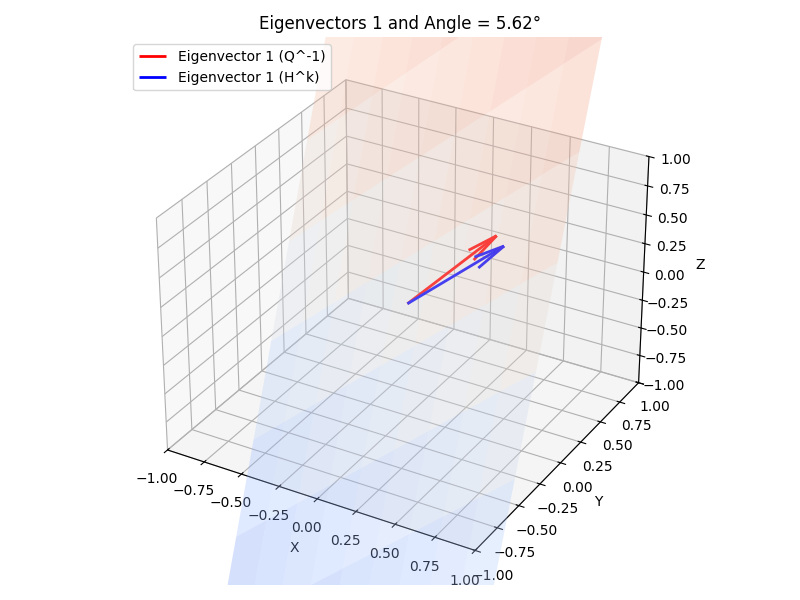
\includegraphics[width=1\textwidth]{eigenvector_pair_1.png}
    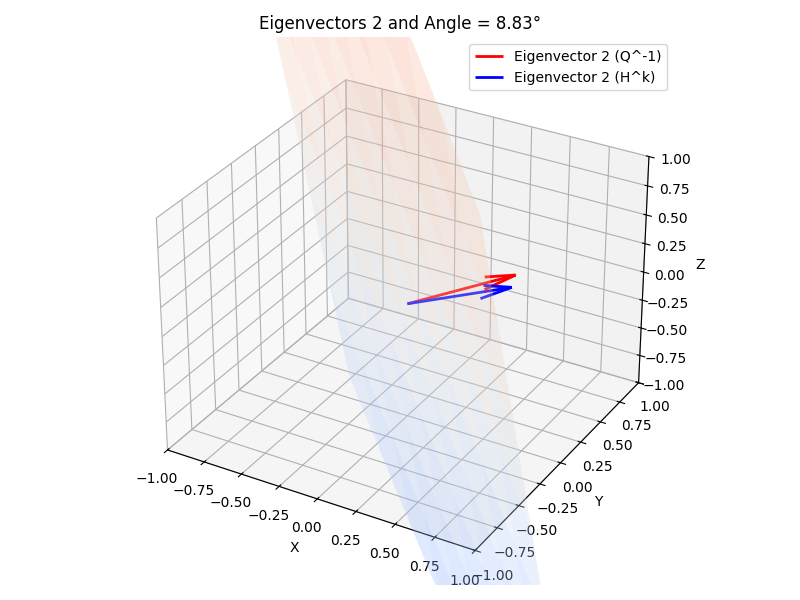
\includegraphics[width=1\textwidth]{eigenvector_pair_2.png}
    

\end{figure}

\begin{figure}[H]
    \centering
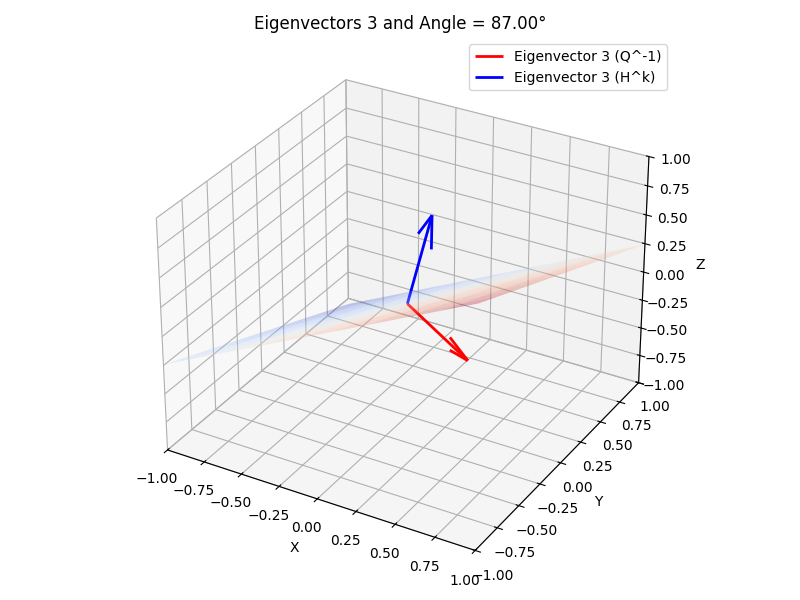
\includegraphics[width=1\textwidth]{eigenvector_pair_3.png}
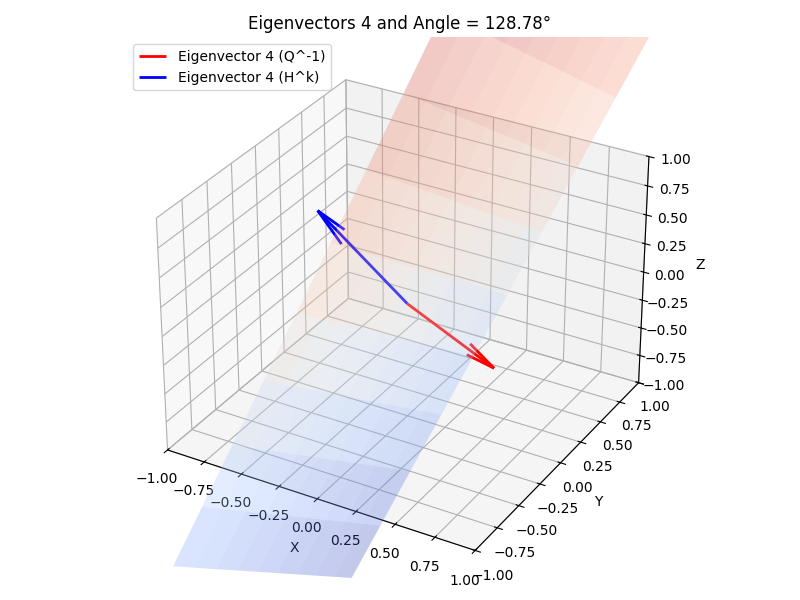
\includegraphics[width=1\textwidth]{eigenvector_pair_4.png}
\end{figure}

\begin{figure}[H]
    \centering
    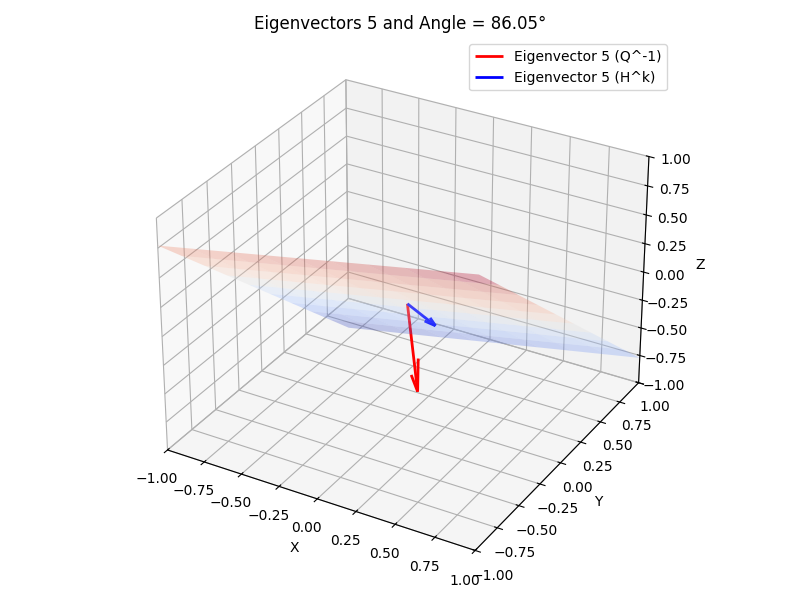
\includegraphics[width=1\textwidth]{eigenvector_pair_5.png}
\end{figure}


\end{document}

